\begin{figure*}[h]
    \centering
    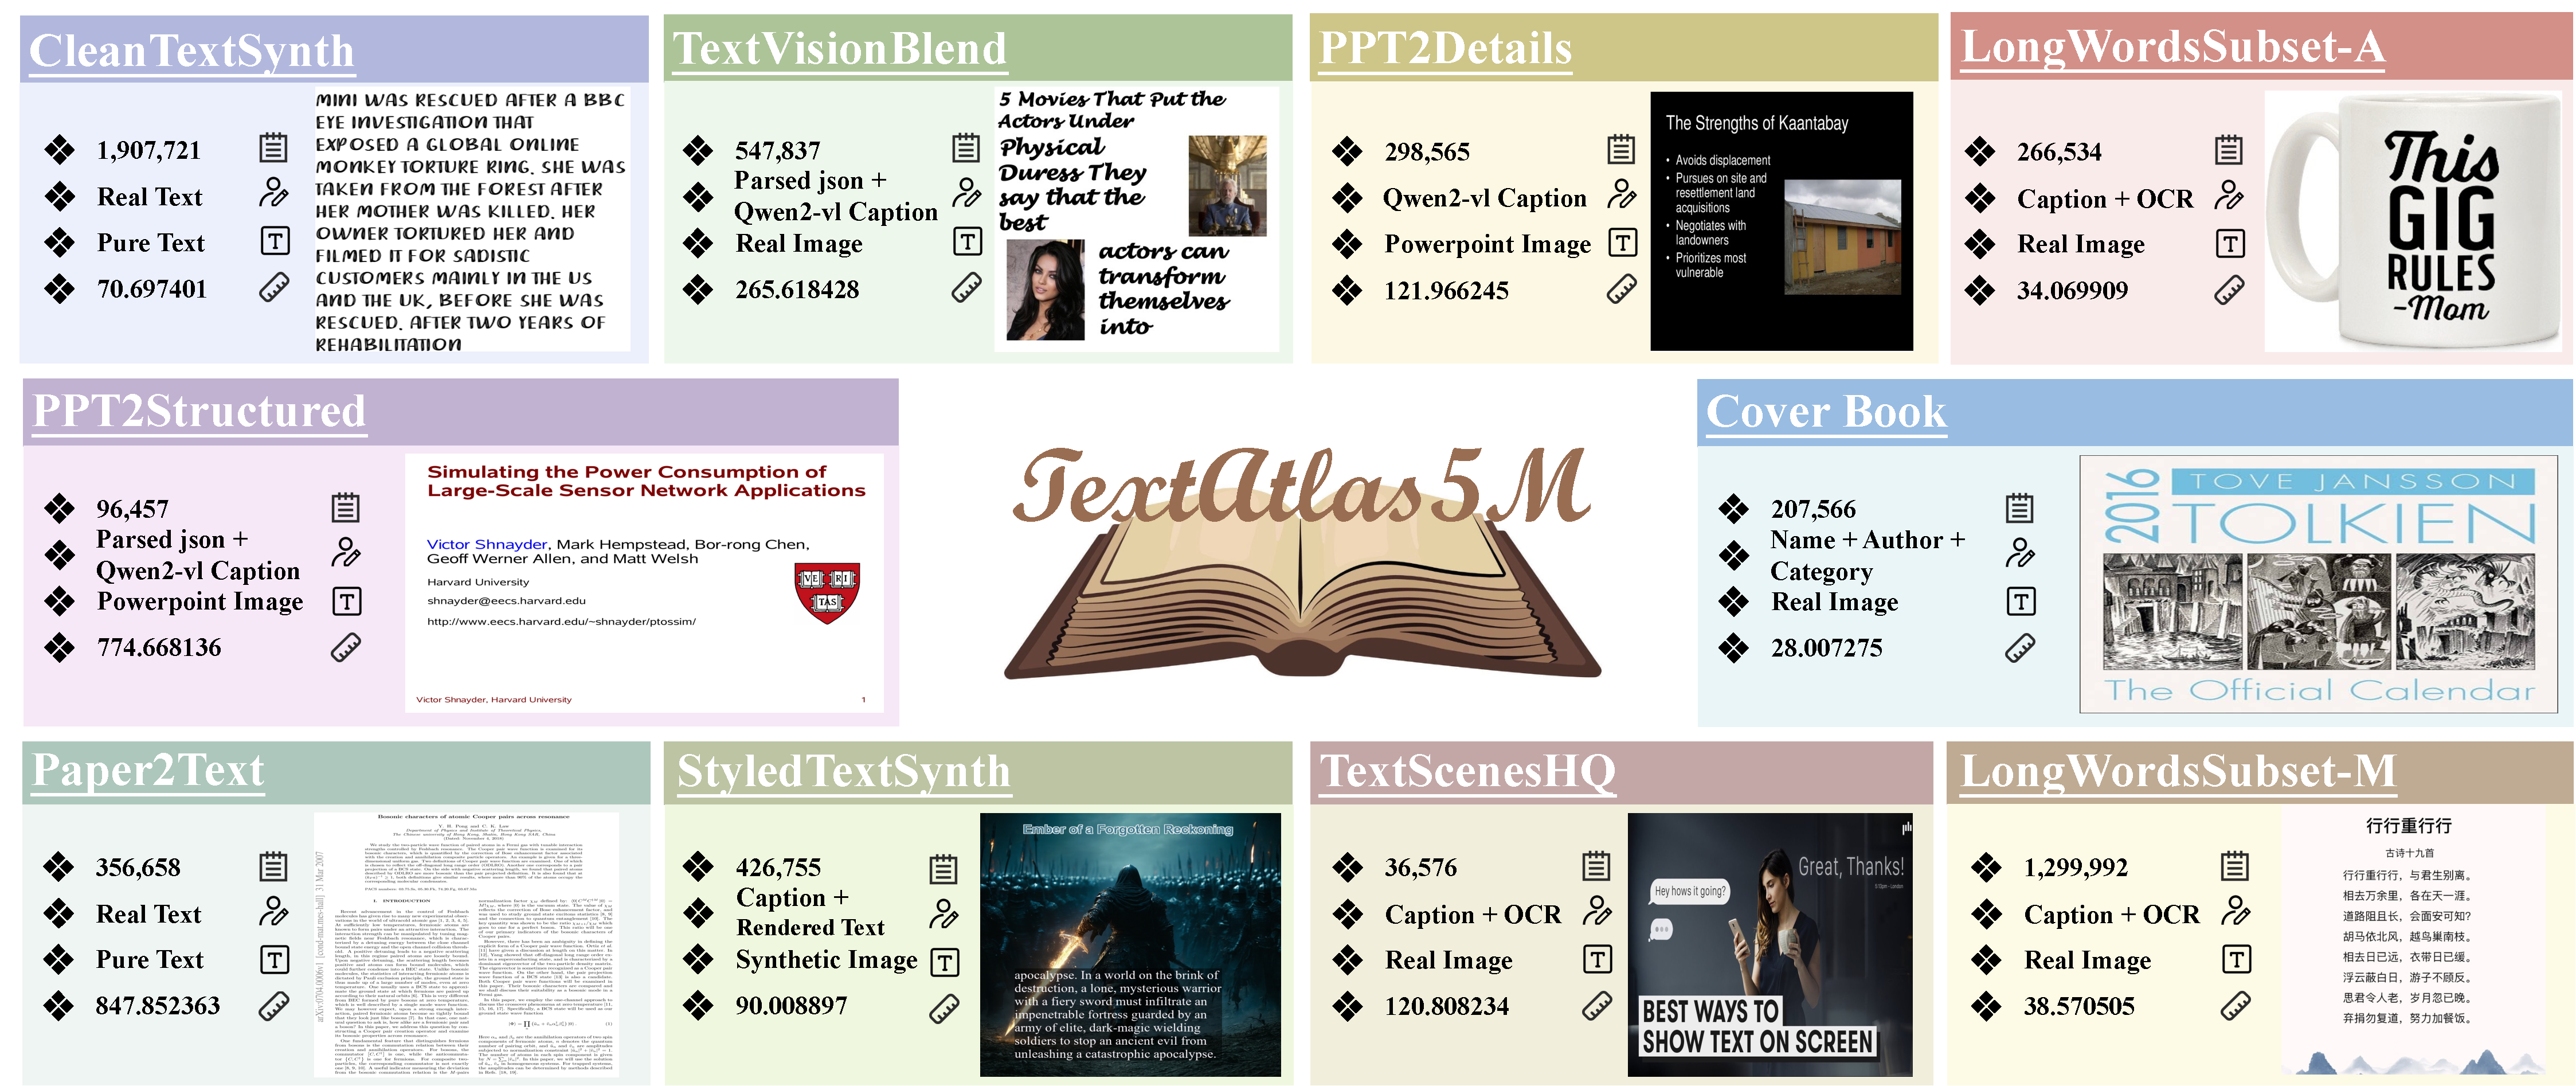
\includegraphics[width=\linewidth]{figures/src/intro_dataset.pdf}
    % \vspace{-4mm}
    \caption{
    \textbf{Overview of \DatasetName Subsets.} 
    \DatasetName\ comprises both Synthetic and Real data splits. 
    The synthetic split features three stages of increasing complexity, from clean text overlays to naturalistic text-image compositions. 
    The real-world split is sourced from a diverse set of domains, capturing authentic dense-text scenarios for robust model evaluation.
    % \textcolor{blue}{Add multi-ling example here.}
    % \textbf{Examples of Subsets in \DatasetName.}
    % The dataset includes Synthetic Data and Real Data splits. 
    % Synthetic data consists of three progressively complex subsets, while real data is gathered from diverse sources.
    }
    % \vspace{-2em}
    \label{fig:all_datasets_visualization}
\end{figure*}